% {{{
\documentclass[a4paper,10pt,english]{article}
\usepackage[utf8]{inputenc}
\usepackage[english]{babel}
\usepackage{graphicx, verbatim, amsmath, amsfonts, geometry, float, import, bm}
\usepackage{siunitx} % converts expression to SI units/notation , \num{10e-10}
\usepackage[hidelinks]{hyperref}
\usepackage{url}
\usepackage{biblatex}


\usepackage{algpseudocode}
\usepackage{algorithm}

% \bibliography{refs}

%Box around tex
\usepackage{mdframed}

%Subfigures
%\usepackage{caption, subcaption}
\usepackage{subfigure}        % imports a lot of cool and useful figure commands

\usepackage{gensymb}


% Code higligthing
\usepackage{listings}
\usepackage{xcolor}
\definecolor{codegreen}{rgb}{0,0.6,0}
\definecolor{codegray}{rgb}{0.5,0.5,0.5}
\definecolor{codepurple}{rgb}{0.58,0,0.82}

\lstdefinestyle{mystyle}{
	commentstyle=\color{codegreen},
	keywordstyle=\color{magenta},
	stringstyle=\color{codepurple},
	basicstyle=\ttfamily\footnotesize,
	breakatwhitespace=false,         
	breaklines=true,                 
	captionpos=b,                    
	keepspaces=true,                 
	numbersep=5pt,                  
	showspaces=false,                
	showstringspaces=false,
	showtabs=false,                  
	tabsize=4
}
\lstset{style=mystyle}
\setlength{\parindent}{0mm}
\setlength{\parskip}{1.5mm}

% }}}

\title{Exploring advantages/disadvantages of solving PDEs with Neural Networks}
\author{Tor-Andreas Bjone}

\begin{document}
\maketitle
\tableofcontents

\begin{abstract}                          % marks the beginning of the abstract

We looked at the mean squared error of several neural networks and an explicit
solver against a closed-form solution. We found that the neural network that
performed best was using the ReLu activation function, the RMSprop otimizer and
had 3 hidden layers. But this had a MSE of 2 orders of magnitude higher than
the explicit solver after 20 epochs. We then timed the explicit solver against a already
trained network for different matrix sizes and found that the explicit solver
was about two orders of magnitude faster than the neural network. For such a
simplistic problem a traditional solver performs better than a neural network.
\end{abstract}                            % marks the end of the abstract

\section{Introduction}
\begin{comment}
In this report we will look at ...
Motivate the reader, the first part of the introduction gives always a
motivation and tries to give the overarching ideas. What I have done. 
The structure of the report, how it is organised. Explain structure of the rapport at the end of intro. 
\end{comment}

In recent years the applications of Neural Networks have been expanded
massively. There has been done a lot of research into solving PDEs with Neural
Networks, such as the paper (Zobeiry \& Humfeld, 2020)\cite{2}.
Solving/approximating such
systems as the Schrödinger equation or the Navier-Stokes equation with no
closed-form solutions can be very beneficial. 

In this report we will tackle a simple problem, the heat equation in 1D, to see how a Neural Network
performs against a conventional numerical method, the Forward Time Central
Space (FTCS) scheme. To evaluate the methods we choose a boundary condition with a closed-form
solution and look at the difference between this and our numerical solutions.
And to set up the Neural Network we use Keras, which is a TensorFlow API.


The method section first goes trough through the closed-form solution and then
the Neural Network. And the results start by comparison of the mean squared
error (MSE) before looking at the time it takes to solve using the explicit
method versus the Neural Network.


\section{Theory and Methods}

\subsection{Heat equation}
We will look at the heat equation in one dimension.
\begin{equation}
    \frac{\partial^2 u(x,t)}{\partial x^2} =\frac{\partial u(x,t)}{\partial t},
    t\geq 0, x\in [0,L]
\end{equation}
or
\begin{equation}\label{eq:heat_eq}
    u_{xx} = u_t,
\end{equation}
with initial conditions
\begin{equation}\label{eq:boundary_x}
    u(x,0)= \sin{(\pi x)} \hspace{0.5cm} 0 \leq x \leq L,
\end{equation}
and with $L=1$ being the length of the $x$-region of interest. The 
boundary conditions are
\begin{align}\label{eq:boundary_t}
    u(0,t) &= 0 \hspace{0.5cm} t \ge 0,\\
    u(L,t) &= 0 \hspace{0.5cm} t \ge 0.
\end{align}

\subsubsection{Closed-form solution}
The analytical solution to this problem is derived in (Tveito and
Winther, 2005, pp. 90-92)\cite{1}, so we will just present a small
summary of the method here. First we assume that $u(x,t)$ is linear and homogeneous and 
that the equation is separable in the form of $u_k(x,t)=X_k(x)T_k(t)$, where
$k$ refers to it being a particular solution. We can then solve the equation 
by separation of variables to find
\begin{equation*}
    u(x,t)_k=e^{-(k\pi/L)^2t}\sin{\left(\frac{k\pi}{L}x\right)},\ k=1,2,3,..
\end{equation*}
This will then give the family ${u_k}$ of particular solutions. We assume then
that $f(x)$ can be written as a linear combination of the eigenfunctions of
$X(x)$, so that
\begin{equation*}
    f(x)=\sum_{k=1}^{N} c_k \sin{\left(\frac{k\pi}{L}x\right)},
\end{equation*}
where $c_k$ is some constant. Then it follows by linearity that
\begin{equation*}
u(x,t)=\sum_{k=1}^N c_ke^{-(k\pi/L)^2t}\sin{\left(\frac{k\pi}{L}x\right)}.
\end{equation*}

Now inserting that $f(x)=\sin(\pi x)$ and $L=1$ it is easy to see that this
gives $c_1=1$ and all other constants $c_k=0$. This gives us the \textbf{closed-form
solution} of
\begin{equation*}
    u(x,t)=e^{-\pi^2 t}\sin{\left(\pi x\right)}.
\end{equation*}

\subsubsection{Numerical approximation}
We will solve this by so called FTCS-scheme (Forward Time Central Space) and
use the Forward-Euler method for moving in time. This results in

\begin{equation*}
u_t\approx \frac{u(x,t+\Delta t)-u(x,t)}{\Delta t}=\frac{u(x_i,t_j+\Delta t)-u(x_i,t_j)}{\Delta t}
\end{equation*}
and
\begin{equation*}
u_{xx}\approx \frac{u(x+\Delta x,t)-2u(x,t)+u(x-\Delta x,t)}{\Delta x^2},
\end{equation*}
or
\begin{equation*}
    u_{xx}\approx \frac{u(x_i+\Delta x,t_j)-2u(x_i,t_j)+u(x_i-\Delta x,t_j)}{\Delta x^2}.
\end{equation*}
And to simplify notation, let
\begin{equation*}
    u(x_i, t_j + \Delta t)\rightarrow u_{i,j+1},
\end{equation*}
and
\begin{equation*}
    u(x_i+\Delta x, t_j) \rightarrow u_{i+1, j}.
\end{equation*}

Then we re-write the equation as

$$
    \frac{u_{i,j+1}-u_{i,j}}{\Delta t} = \frac{u_{i+1,j}+u_{i-1,j}-2u_{i,j}}{\Delta
    x^2}.
$$
Now we can define $\alpha=\Delta t / \Delta x^2$ to get

\begin{equation}
    u_{i,j+1}=\alpha u_{i-1,j} + (1-2\alpha) u_{i,j}+\alpha u_{i+1,j},
\end{equation}

Where we have discretized $x$ and $t$ so that
$$
    x_i = i\Delta x,\ i=0,1,2,...,n,
$$
and
$$
    t_j = j\Delta t,\ j=0,1,2,...,m.
$$

And this scheme is only numerically stable when the \textbf{Von Neumann
stability criterion} is met:
$$
    \alpha\leq 1/2,
$$ 
as described in (Tveito and
Winther, 2005, pp. 132-133)\cite{1}. And it has a \textbf{truncation
error} of
$O(\Delta x^2)$ (Tveito and Winther, 2005, p. 64)\cite{1}.

We note that this problem can be reduced to solving a matrix system, where
$$
    A=
    \begin{bmatrix}
        1-2\alpha & \alpha & 0 & 0 & ... & 0 \\
        \alpha    & 1-2\alpha & \alpha & 0 ... & 0 \\
        0 & \alpha & 1-2\alpha & \alpha & 0 & ... \\
        ... & ... & ... & ... & ... & ... \\
        0 & ... & ... & 0 & \alpha & 1-2\alpha
    \end{bmatrix}
$$
is a tri-diagonal Topelitz matrix. And we can define a column vector for the
time step as
$$
    V_j = 
    \begin{bmatrix}
        u_{1,j}\\
        u_{2,j}\\
        ...\\
        u_{n,j}
    \end{bmatrix}
$$
so that
\begin{equation}
    V_{j+1} = AV_j.
\end{equation}

And this can be Forward solved using the Toeplitz forward solver algorithm \ref{algo:toeplitz}.

\begin{algorithm}
    \caption{Toeplitz Forward solver algorithm}\label{algo:toeplitz}
    \begin{algorithmic}
        \Require{Spacial step-size $\Delta x$}
        
        \Require{Timespan $T$ and lengthspan $L$.}
        
        \Require{Stability criterion parameter $\alpha$.}
        
        \Require{Function f(x)=u(x,0).}
        
        Calculate diagonal elements: $a=\alpha$, $b=1-2\alpha$.
    
        Calculate first timestep $u(x,0)=f(x)$ and set boundary conditions.
    
        \While{Time is less than $T$}
            
            $u(x, t+\Delta t) = a \cdot u(x-\Delta x, t) + b\cdot u(x,
            t) + a \cdot u(x+\Delta x, t)$.
    
            Set boundary conditions.
        \EndWhile
    
    \end{algorithmic}
    \end{algorithm}
    
    This is a
    method of solving a tri-diagonal matrix system without having to do the matrix
    multiplication. 
    
    For our program we have chosen to hold the entire solution in space and time in
    memory. But it is also possible to iterate in time without holding in memory
    and just save the time-steps you want to look at. But for the 1D case this is
    not a concern on a modern computer as we will look at arrays with a maximum of
    $10^4\times 10^4$, which will be under one Megabyte with 32-bit numbers.
   
\subsection{Solving with Neural Networks}
We will use the \textbf{keras API for TensorFlow} to approximate the heat
equation with a NN. To train the network we will use the analytical solution
with the mean squared error as the cost function. This is done by creating a
matrix $X$ that holds all $x$ and $t$ values and a matrix $u$ with the
corresponding analytical values. We will let $x$ be of length $n=100$ and $t$
be of length $m=100$ for the training of the network. Then for the testing we
will double the size of $n$ and $m$. We do not need to shuffle the dataset or
do a train/test split when testing in this way, although some of the training
set will be included in the test set when doing it this way. This will not matter
as we increase the size of the dataset for the testing and will therefore be
able to spot overfitting if it should happen.

We will set up the network
with 3 hidden layers, with 16 neurons in the first layer, then 32 neurons in
the following two layers. This will be tested using the Adam and RMSprop
optimizers, and ReLu and Sigmoid activation functions. Then we will take the
best performing of these and increase the complexity of the network by adding
new layers of 32 neurons. These will all be trained using a batch size of 30
and 20 epochs.

Then we will look at the time the trained network uses for giving out a
prediction, or feed forwarding, for a two layer network versus the explicit solver. 
Where this network has been trained using RMSprop and has ReLu activation functions.






\begin{comment}
But since the exact solution will
most likely not be reached we can instead try to minimize the given conditions
of the equation. We re-write the heat equation and the boundaries as a minimization problem
\begin{equation*}
    \min_{x,t} \left\{
    \lVert \hat u_{xx} - \hat u_t \rVert^2 
    + \lVert \hat u(0,t) \rVert^2 
    + \lVert \hat u(1,t) \rVert^2
    + \lVert \hat u(x,0)-\sin{(\pi x)}\rVert^2 \right\},
\end{equation*}
where this norm $\lVert \cdot \rVert$ is to be read as the grand sum of the
matrix. We then define our cost/loss-function as
\begin{equation*}
    C(\hat u) =\frac{1}{2} \left[ \lVert \hat u_{xx} - \hat u_t \rVert^2 
    + \lVert \hat u(0,t) \rVert^2 
    + \lVert \hat u(1,t) \rVert^2
    + \lVert \hat u(x,0)-\sin{(\pi x)}\rVert^2 \right]
\end{equation*}

For the backpropagation of our network we need the derivative of this with
respect to the output of the network, which is $\hat u$.
\begin{equation*}
    \frac{\partial C}{\partial\hat u} = 
\end{equation*}
\end{comment}

\section{Results and Discussion}

\begin{figure}[h!]
    \centering
    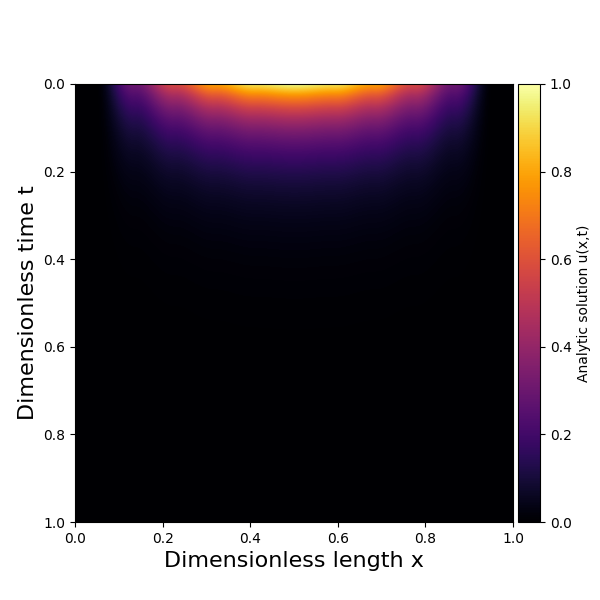
\includegraphics[width=8cm]{../Figures/analytic_solution.png}
    \caption{Analytic solution for the heat equation with initial conditions
    $u(x,0)=\sin{(\pi x)}$ and boundary conditions $u(0,t)=u(1,t)=0$.}
    \label{fig:analytic_solution}
\end{figure}

In figure \ref{fig:analytic_solution} we see the analytic solution for our
given boundary and initial conditions. This will be used to test our numerical
solvers using the absolute error between this and the numerical approximation.
This can be seen in figure \ref{fig:abs_error_all}. In the subfigures (a)-(d)
we see the NNs prediction for different activation functions and optimizers. We
can see that ReLu with RMSprop has the lowest error. And we note that all of
the approximations have the highest loss at the boundaries. We can especially
see that Adam with ReLu has a very high error at the $t=0$ boundary. The reason
our network is not handling the boundaries well is because the loss function
has no special penalizing of wrong boundaries. This could be fixed by creating
a new loss function by looking at the minimization of the NNs prediction

\begin{equation*}
    \min_{\hat{u}} \left\{
    \lVert \hat u_{xx} - \hat u_t \rVert^2 
    + \lVert \hat u(0,t) \rVert^2 
    + \lVert \hat u(1,t) \rVert^2
    + \lVert \hat u(x,0)-\sin{(\pi x)}\rVert^2 \right\},
\end{equation*}
where this norm $\lVert \cdot \rVert$ is to be read as the grand sum of the
matrix. We then define our cost/loss-function as
\begin{equation*}
    C(\hat u) =\frac{1}{2} \left[ \lVert \hat u_{xx} - \hat u_t \rVert^2 
    + \lVert \hat u(0,t) \rVert^2 
    + \lVert \hat u(1,t) \rVert^2
    + \lVert \hat u(x,0)-\sin{(\pi x)}\rVert^2 \right].
\end{equation*}
We can then add parameters in front of the norms to decide how costly it would
be for the network to not prioritize the boundaries. This is called a physics
informed neural network and has been explored in a previous paper (Zobeiry \&
Humfeld, 2020)\cite{2}. Getting back to figure \ref{fig:abs_error_all}, we look
at the explicit solver in (e). Note here that the limits on the colorbar is
changed because the error is so small compared to that of the NNs. We see that
now our boundaries is forced to be correct. And we can see that as we move in
time the middle of the rod gets a larger and larger error until it starts
cooling down and of course the error gets smaller because the values get closer
and closer to zero because of the $u(0,t)=u(1,t)=0$ boundaries.

!!!YOU STOPPED HERE!!! Next is loss vs epochs for all methods. Then loss vs
layers. Then time vs matrixsise


\begin{figure}
\centering
\subfigure[Rms, ReLu]{\label{fig:a}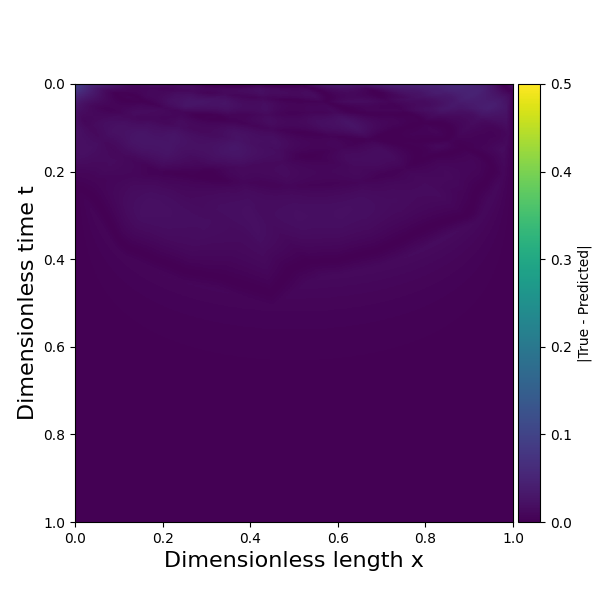
\includegraphics[width=70mm]{../Figures/error_rms_relu.png}}
\subfigure[Rms, Sigmoid]{\label{fig:b}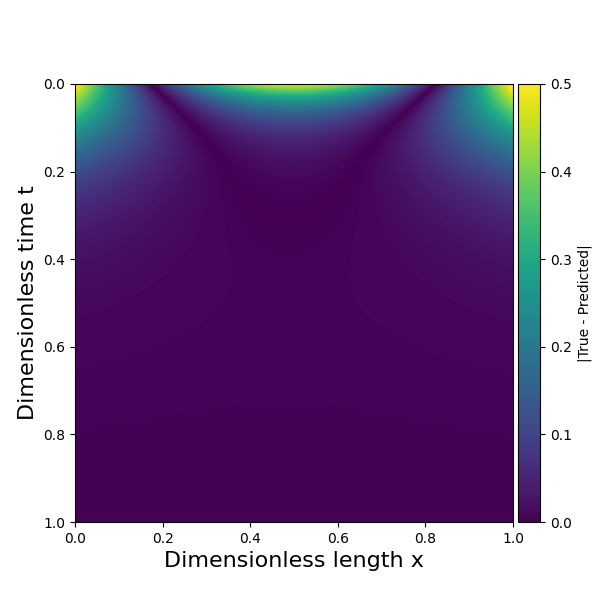
\includegraphics[width=70mm]{../Figures/error_rms_sigmoid.png}}
\subfigure[Adam, ReLu]{\label{fig:c}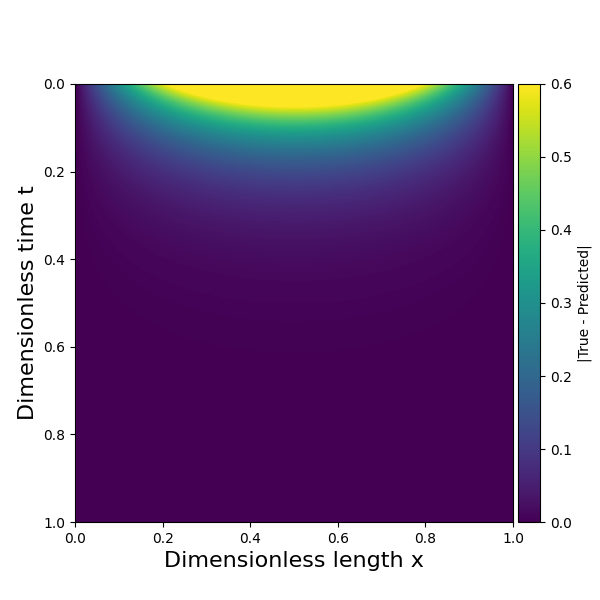
\includegraphics[width=70mm]{../Figures/error_adam_relu.png}}
\subfigure[Adam, Sigmoid]{\label{fig:d}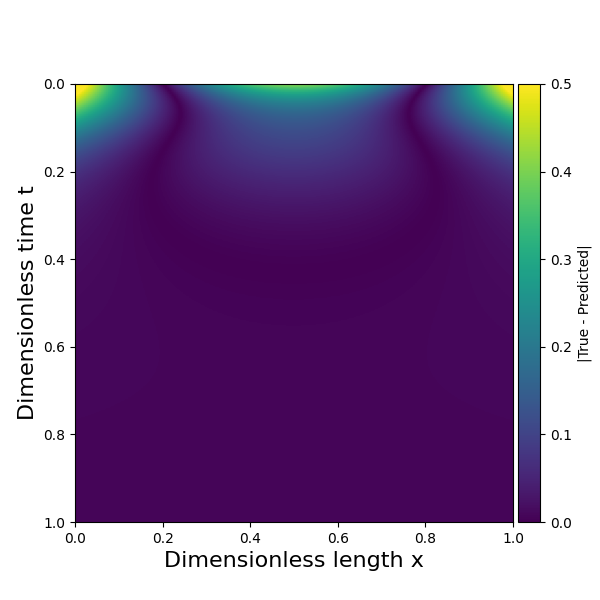
\includegraphics[width=70mm]{../Figures/error_adam_sigmoid.png}}
\subfigure[Explicit solver]{\label{fig:e}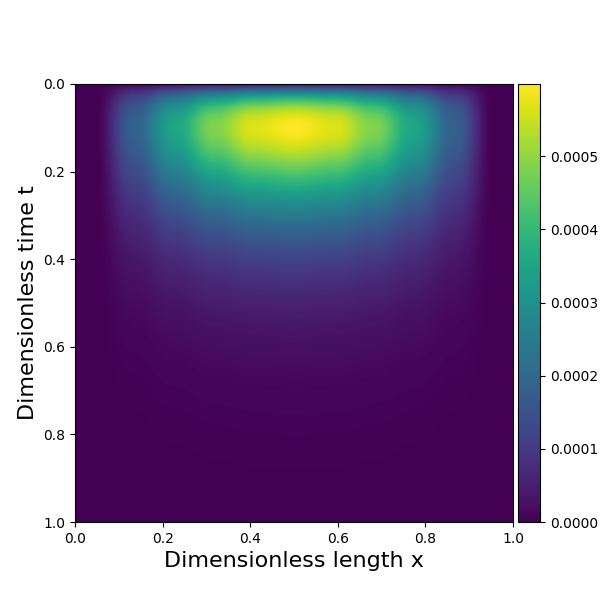
\includegraphics[width=70mm]{../Figures/error_explicit.png}}
\caption{Absolute error for NN in (a)-(d) and explicit solver in (e). NN is
trained with 20 epochs and a batch size of 30 with $(n=100)\times (m=100)$
data points of $x$
and $t$ respectively, using the analytical solution for MSE as the loss
function. The explicit solver in (e) is using $\Delta x=0.1$ and $\alpha=1/4$.}
\label{fig:abs_error_all}
\end{figure}

\section{Conclusion}
\begin{comment}
State your main findings and interpretations. 
Try as far as possible to present perspectives for future work. 
Try to discuss the pros and cons of the methods and possible improvements.
\end{comment}

For the Neural Network we found that the simpler networks performed better on
this problem. Specifically a 3 layer network trained using RMSprop, with ReLu
activation functions performed best in terms om the MSE against the analytical
solution. But we found that the explicit solver performed better, with about
two-three orders of magnitude lower MSE. This is mostly because of the boundary
conditions, as there is no implementation in the networks to penalize high MSE
on the boundaries. For future work we could create a cost function for the
network as described in the previous section, by looking at the minimization
problem of the heat equation and the boundary conditions.

We also found that the time the already trained network used to predict a
solution was about two orders of magnitude slower than the time used for the
explicit solver. This indicates that for such a simple problem there is no
benefits to using a Neural Network. For future work one could also look at
implicit schemes such as Crank-Nicolson, which is stable for all $\Delta x$ and
$\Delta t$ and could possibly solve even faster. 

One could imagine that as the complexity of the problem increased the Neural
Network would perform better compared to the explicit scheme. Therefore it
would be beneficial to look at the heat equation in 2D and 3D. And if we have a
cost function that is not based on an analytical solution, we could train the
network with ICs as parameters and see if the network can predict for ICs that
it has not been trained on. In that case one could solve problems without
closed-form solutions.





\section*{References}  
\begin{itemize}
\bibitem[1]{1} Tveito, A. \& Winther, R. (2005) Introduction to Partial Differential Equations: A computational approach. 2nd edn. New York, NY, USA: Springer.

\bibitem[2]{2} Humfeld, K \& Zobeiry, N. (2020)  Physics-Informed Machine Learning Approach for Solving Heat Transfer Equation
    in Advanced Manufacturing and Engineering Applications. Washington, Seattle, WA: University of Washington
\end{itemize}



\begin{figure}
\centering
\subfigure[Rms, ReLu]{\label{fig:a}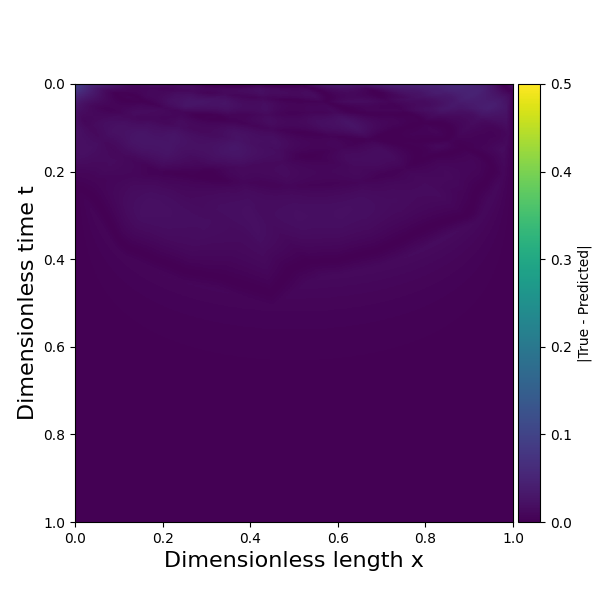
\includegraphics[width=70mm]{../Figures/error_rms_relu.png}}
\subfigure[Rms, Sigmoid]{\label{fig:b}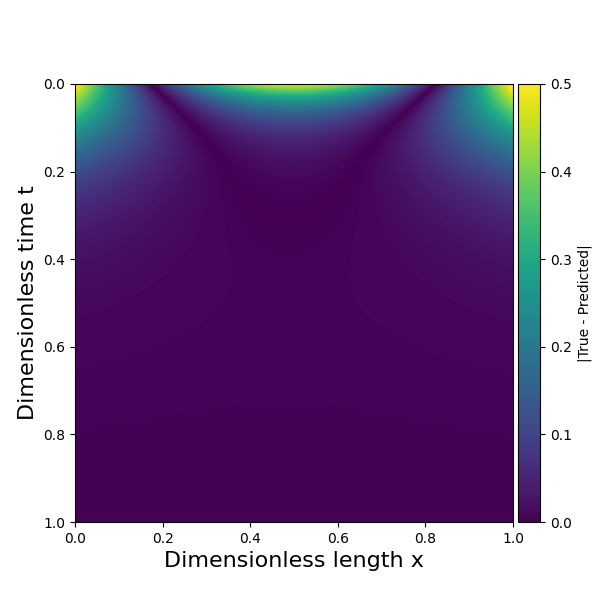
\includegraphics[width=70mm]{../Figures/error_rms_sigmoid.png}}
\subfigure[Adam, ReLu]{\label{fig:c}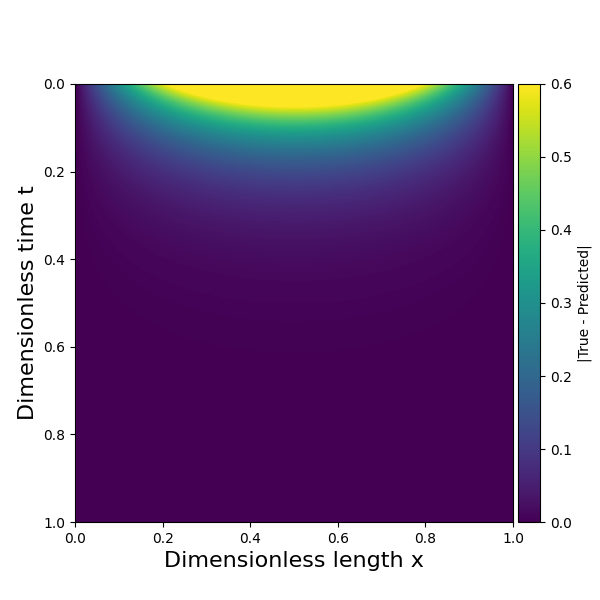
\includegraphics[width=70mm]{../Figures/error_adam_relu.png}}
\subfigure[Adam, Sigmoid]{\label{fig:d}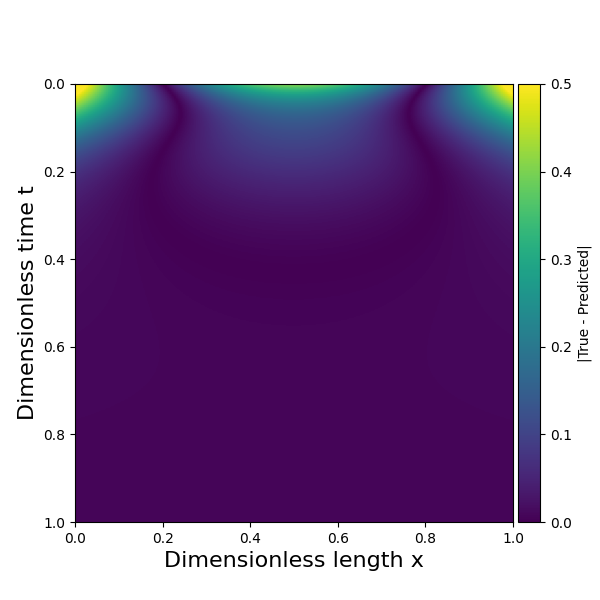
\includegraphics[width=70mm]{../Figures/error_adam_sigmoid.png}}
\subfigure[Explicit solver]{\label{fig:e}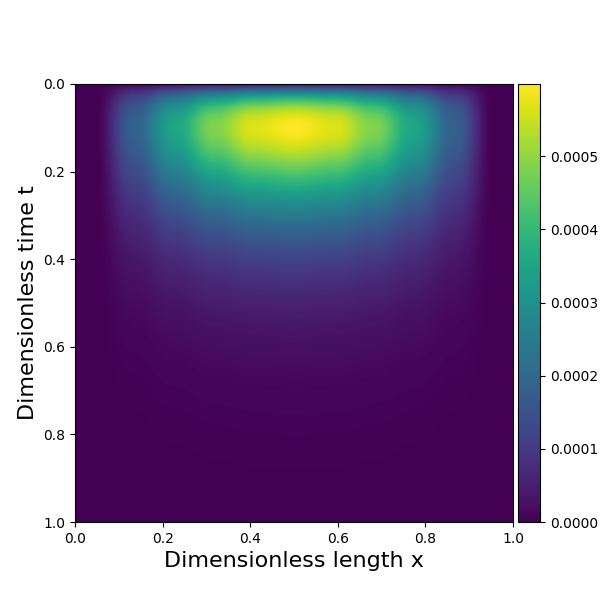
\includegraphics[width=70mm]{../Figures/error_explicit.png}}
\caption{Absolute error for NN in (a)-(d) and explicit solver in (e). NN is
trained with 20 epochs and a batch size of 30 with $(n=100)\times (m=100)$
data points of $x$
and $t$ respectively, using the analytical solution for MSE as the loss
function. The networks have three hidden layers, one of 16 neurons and two of 32.
The explicit solver in (e) is using $\Delta x=0.1$ and $\alpha=1/4$.}
\label{fig:abs_error_all}
\end{figure}



\end{document}
